\section{Problem Delimitation}
During the problem analysis, multiple areas of big data and grid computing have been explored. This was done to specify a focus area of the initial problem statement. A concept map was created to get an overview of the different problems that exist when working with big data and problems related to grid computing. This is what is shown in figure \ref{fig:concept_map}. As seen in the initial problem statement, the focus was initially on developing a grid computing system where an implementation of a sorting algorithm would be created, that would also verify the correctness of the given result. During the process analysis, the scope and relevance of these areas were discovered. Because of this, one area was chosen to focus on. The only part that will be focused on in this project is the sorting part of the grid computing system and validation will not be a focus.


\begin{figure}[H]
    \centering
    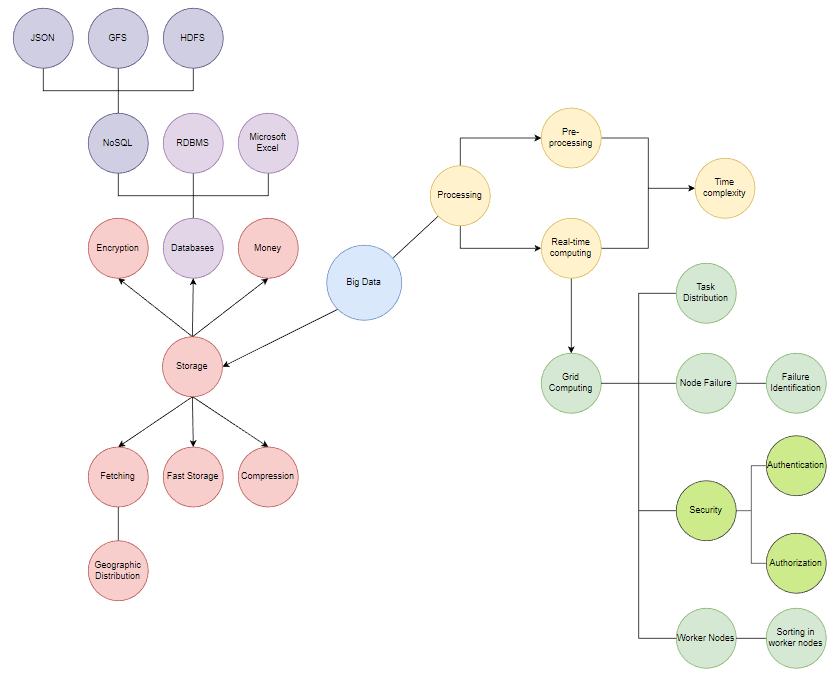
\includegraphics[scale=0.95]{figures/concept_map.png}
    \caption{Concept map of problems regarding big data.}
    \label{fig:concept_map}
\end{figure}